\documentclass[fr]{../../../eplsummary}

\usepackage{float}
\usepackage{colonequals}

\graphicspath{{img/}}

\newcommand{\prop}{\langle \textnormal{proposition} \rangle}
\newcommand{\impdef}{\mathrel{\ratio \hskip -2\mu \coloneqq}}
\newcommand{\true}{\textnormal{true}}
\newcommand{\false}{\textnormal{false}}
\newcommand{\EP}{\mathcal{E}_P}
\newcommand{\val}[1]{\mathrm{val}_{#1}}
\newcommand{\VAL}[1]{\mathrm{VAL}_{#1}}
\newcommand{\tauto}{{\vDash} \>}
\newcommand{\contra}{{\nvDash} \>}

\hypertitle{Logique et structures discrètes}{5}{INGI}{1101}
{Gilles Peiffer}
{Peter Van Roy}

\section{Contexte: la méthode scientifique}
La logique est la science du raisonnement.
Il existe 3 types de raisonnement:
\begin{itemize}
	\item la déduction\footnote{Qu'on étudiera dans ce cours.};
	\item l'induction;
	\item l'abduction.
\end{itemize}
Tout raisonnement fait par un humain
fait partie de l'une de ces trois catégories.
Prenons l'exemple de la méthode scientifique.
L'humain commence en général par émettre une théorie
sur comment fonctionne le monde,
et ce en se basant sur un modèle théorique du monde réel.
Ensuite, à partir de cette théorie,
il est possible de \emph{déduire} les résultats
que devrait avoir une certaine expérience,
si la théorie est juste.
On effectue alors l'expérience,
et on \emph{induit} à partir des résultats
une règle que semble suivre la nature.
Finalement, observant cette règle naturelle,
on la compare avec la théorie proposée,
et si les deux ne sont pas en accord,
on se pose la question ``Pourquoi la nature suit-elle cette règle?''.
La réponse à cette question est une abduction.
\begin{figure}[H]
	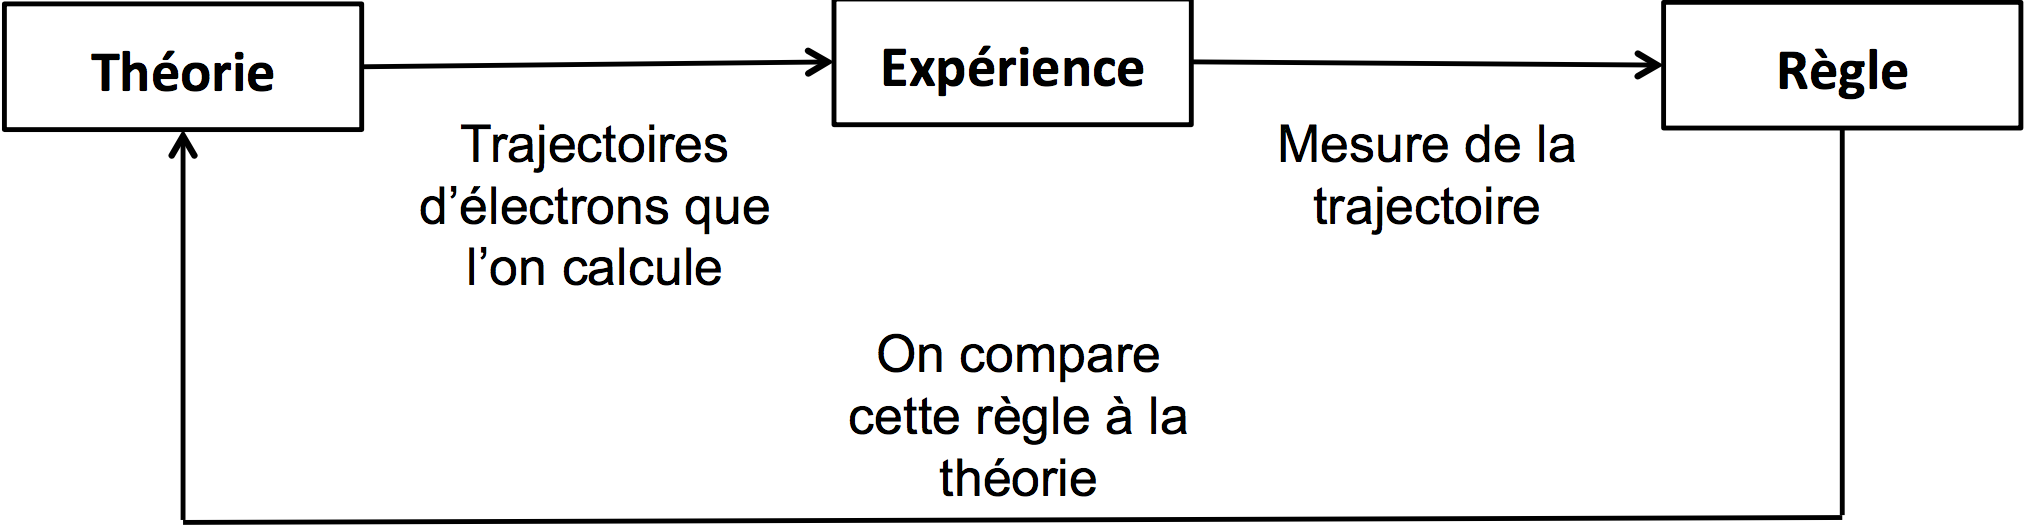
\includegraphics[width=\textwidth]{scientific_method}
	\caption{Un exemple d'utilisation de la méthode scientifique
	pour les lois de Maxwell.
	Notons que ce schéma n'est pas entièrement complet:
	il faudrait séparer la partie ``Expérience'' en deux;
	d'une part tout ce qui est prédiction,
	et d'autre part la mise en place.
	La théorie permet alors de faire les deux.}
	\label{fig:sci_meth}
\end{figure}
\bigbreak
On remarque donc que sur ces trois raisonnements,
uniquement la déduction est un raisonnement sûr,
alors que l'induction et l'abduction ne le sont pas.
\begin{myexem}[Sac de billes]
Un exemple illustrant cette différence
serait un sac rempli de billes colorées.
On suppose que la théorie nous dit
que toutes les billes sont blanches.
On \emph{déduit} donc avec parfaite sûreté
que si on pioche une bille du sac,
elle sera blanche.

Comparons cela avec le cas suivant:
on est en train de piocher des billes du sac,
et on remarque que toutes les billes que l'on pioche sont blanches.
On peut alors \emph{induire} que toutes les billes du sac sont blanches.
Ce raisonnement n'est pas parfaitement sûr,
contrairement à la déduction.

Finalement, supposons que l'on trouve un bille blanche à coté du sac.
On pourrait expliquer cela par le fait que les billes viennent du sac.
Il s'agit d'un raisonnement abductif,
qui n'est d'ailleurs pas sûr.
\end{myexem}

\section{La logique propositionnelle}
La logique propositionnelle
est la plus simple des formes de logique
(on a également la logique des prédicats\footnote{Plus tard dans le cours\dots},
la logique du second ordre, la logique temporelle, la logique modale,\dots).
Elle permet de formaliser les connexions logiques entre des propositions.
\bigbreak
\begin{mydef}[Proposition première]
	Les \emph{propositions premières} sont les ``briques''
	avec lesquelles nous construisons les propositions plus compliquées.
	Elle peut soit être vraie (true) ou fausse (false).
	Un exemple pourrait être la phrase
	``La logique est compliquée\footnote{En l'occurrence,
	cette proposition est fausse\dots}.''
	On les dénote avec des lettres majuscules ($A$,$B$,\dots).
\end{mydef}
\begin{mydef}[Proposition logique]
	Une \emph{proposition logique} est alors soit une proposition première,
	soit une combinaison de propositions logiques
	connectées par des connecteurs logiques.
\end{mydef}
L'avantage de cette notation est qu'elle permet de raisonner formellement
sur les propositions logiques.
On peut définir:
\begin{enumerate}
	\item une \emph{syntaxe} (définie par une grammaire)
	qui définit ce qui est une proposition logique et ce qui ne l'est pas;
	\item une \emph{sémantique}
	qui donne un sens à chaque proposition logique;
	\item une \emph{théorie de preuve} permettant,
	en sachant qu'une proposition est vraie,
	de trouver d'autres propositions vraies.
\end{enumerate}
\subsection{Syntaxe}
\label{sec:syntax}
La logique propositionnelle est un \emph{langage formel}.
Ce langage peut être défini à l'aide d'une grammaire sur un \emph{alphabet}.
Cet alphabet est l'ensemble des symboles qui composent une proposition logique:
\begin{itemize}
	\item les lettres majuscules pour les propositions premières: $A$,$B$,\dots;
	\item true et false pour les propositions
	resp. toujours vraie et toujours fausse;
	\item les connecteurs logiques:
	\begin{itemize}
		\item la conjonction (AND): $\land$;
		\item la disjonction (OR): $\lor$;
		\item la négation (NOT): $\lnot$;
		\item l'implication: $\to$ ou $\implies$;
		\item l'équivalence: $\leftrightarrow$ ou $\iff$;
		\item les caractères de ponctuation: $($ et $)$.
	\end{itemize}
\end{itemize}
La grammaire suivante permet de donner les règles
que doivent respecter les phrases propositionnelles:
\[
\renewcommand{\arraystretch}{1.5}
\begin{array}{rrl}
	\langle \textnormal{identificateur} \rangle & \impdef & A \mid B \mid C \mid \dots\\
	\prop &\impdef& \true\\
	&\mid& \false\\
	&\mid& \langle \textnormal{identificateur} \rangle\\
	&\mid& \big(\prop\big)\\
	&\mid& \lnot \prop\\
	&\mid& \prop \land \prop\\
	&\mid& \prop \lor \prop\\
	&\mid& \prop \to \prop\\
	&\mid& \prop \leftrightarrow \prop
\end{array}
\]
On remarque qu'uniquement les séquences de symboles
qui respectent cette grammaire
sont des phrases propositionnelles.
\paragraph{Métalangage}
Le métalangage est un deuxième langage utilisé pour parler d'un premier,
dans notre cas, la logique propositionnelle.
Notre métalangage est le français,
auquel on ajoute les notations mathématiques.
Ce concept est important pour distinguer raisonnement formel et informel.
\subsection{Tables de vérité}
% TODO after second lesson
La syntaxe développée à la section \sectionref{syntax}
permet d'écrire les propositions en logique formelle,
mais ne leur donne pas de sens (vrai ou faux).
Afin de donner un sens aux propositions,
il faut commencer par déterminer
si les propositions premières sont vraies ou fausses.
Pour cela, il y a deux approches:
les \emph{tables de vérité}
et les \emph{interprétations}.
\subsection{Interprétations}
On peut également définir si une proposition est vraie ou fausse
en utilisant une \emph{interprétation}.
Soit $\EP$ l'ensemble des propositions premières.
Alors, une interprétation $I$ définit
une fonction de valuation $\val{I} \colon \EP \to \{\true,\false\}$,
qui permet de savoir si ces propositions premières sont vraies ou fausses\footnote{La notation $f \colon A \to B$ signifie ici
que $f$ est une fonction depuis l'ensemble $A$ vers l'ensemble $B$.}.
On pourrait par exemple écrire
\begin{align*}
	\left\{
	\begin{array}{rcl}
		\val{I_1}(P) & = & \true\,,\\
		\val{I_1}(Q) & = & \false
	\end{array}
	\right.
	\quad \textnormal{et} \quad
	\left\{
	\begin{array}{rcl}
		\val{I_2}(P) & = & \true\,,\\
		\val{I_2}(Q) & = & \true\,.
	\end{array}
	\right.
\end{align*}
Il y a donc différentes interprétations possibles,
et chacune d'elle risque de donner un résultat différent.
\bigbreak
À partir de ces fonctions de valuation premières,
on peut définir d'autres fonctions de valuation:
$\VAL{I}$ se définit par rapport à $\val{I}$.
On a ainsi
\begin{align*}
	\VAL{I}(P) &= \val{I}(P)\,,\quad \forall P \in \EP\,,\\
	\VAL{I}(\lnot P) &=
	\left\{
	\begin{array}{l}
		\false \textnormal{ si } \VAL{I}(P) = \true\,,\\
		\true \textnormal{ sinon}\,,
	\end{array}
	\right.\\
	\VAL{I}(P \land Q) &=
	\left\{
	\begin{array}{l}
		\true \textnormal{ si } \VAL{I}(P) = \true \textnormal{ et } \VAL{I}(Q) = \true\,,\\
		\false \textnormal{ sinon}\,,
	\end{array}
	\right.\\
	\VAL{I}(P \lor Q) &=
	\left\{
	\begin{array}{l}
		\true \textnormal{ si } \VAL{I}(P) = \true \textnormal{ ou } \VAL{I}(Q) = \true\,,\\
		\false \textnormal{ sinon}\,.
	\end{array}
	\right.
\end{align*}
\subsection{Les modèles logiques}
Une interprétation est un modèle $M$ pour une certaine théorie si
les propositions premières sont telles
que tous les axiomes de la théorie soient vrais.
\begin{myexem}
	Prenons le cas suivant:
	\begin{align*}
		&L\textnormal{: ``Le cours de logique est facile.'',}\\
		&E\textnormal{: ``L'étudiant a bien étudié.'',}\\
		&R\textnormal{: ``L'étudiant a réussi l'examen de logique.'',}
	\end{align*}
	\[
	\big(L \land E\big) \to R\,.\tag*{Axiome (1)}
	\]
	Un modèle possible des études supérieures serait donc
	\[
	(L,E,R) = (\true,\true,\true)\,.
	\]
\end{myexem}
On peut donc dire que la théorie est un ensemble de formules
et que le modèle est une interprétation qui satisfait ces formules.
\bigbreak
Soit une formule $p$ aléatoire.
\begin{mydef}[Tautologie]
	Si $p$ est vraie dans toutes les interprétations possibles,
	alors on dit que $p$ est une tautologie ($\tauto p$).
	On a par exemple $p \equiv \big(P \lor \lnot P\big)$.
\end{mydef}
\begin{mydef}[Contradiction]
	Si $p$ est fausse dans toutes les interprétations possibles,
	alors on dit que $p$ est une contradiction ($\contra p$).
	On a par exemple $p \equiv \big(P \land \lnot P\big)$.
\end{mydef}
\begin{mydef}[Contingence]
	Si $p$ n'est ni une tautologie,
	ni une contradiction,
	on dit que $p$ est contingente.
	Par exemple, $p \equiv \big(P \land \lnot Q\big)$.
\end{mydef}
\subsubsection{Conséquence logique}
On note ``$q$ est conséquence logique de $q$''
par $p \models q$.
Si $M$ est modèle de $p$, alors $M$ est aussi modèle de $q$.
\begin{myexem}
	Soit $p \equiv \big(P \land Q\big)$ et $q \equiv \big(P\big)$.
	On a alors que $p \models q$.
\end{myexem}
\end{document}
